\documentclass[10pt]{article} 
%\documentclass{article}
\usepackage{fontspec}
\setmainfont{Times New Roman}

\usepackage{graphicx}
\usepackage{blindtext}
\usepackage{anysize}
    \marginsize{3.175cm}{2.54cm}{1.905cm}{1.905cm} 
\usepackage{appendix}
\usepackage{lastpage}
\usepackage{fancyhdr} 
    \pagestyle{fancy}
    \fancyhf{}
    \fancyhead[L]{\footnotesize Industry EntryLevel-AI powered Industrial
Power Electronics \& Embedded System design}
    \fancyhead[R]{\footnotesize \rightmark} 
    \fancyfoot[C]{\footnotesize 2025-26} 
    \fancyfoot[L]{\footnotesize Dept.of ECE,Vemana IT} 
    \fancyfoot[R]{Page \thepage\ of \pageref{LastPage}}
    \renewcommand{\footrulewidth}{0.4pt}
\usepackage{setspace}  
\usepackage{caption}
\usepackage{chngcntr}
\usepackage{float}
\usepackage{array}
\usepackage{multirow}
\usepackage{booktabs}

\renewcommand{\figurename}{Fig}
\usepackage{chngcntr}
\counterwithin{figure}{section}


\begin{document}
\doublespacing


\newpage
\markright{INTRODUCTION}
\begin{flushleft}
{\fontsize{16pt}{16pt}\selectfont
\section*{CHAPTER 1}}
\end{flushleft}
\begin{center}
{\fontsize{18pt}{18pt}\selectfont \textbf{INTRODUCTION}}
\end{center}
\onehalfspacing
\fontsize{12pt}{14pt}\selectfont
\setlength{\parskip}{6pt}

\noindent
Industrial internships play an important role in engineering education by helping students gain practical    exposure and understand real industrial working environments. They bridge the gap between classroom learning and practical applications by enabling students to observe how theoretical concepts are implemented in industries. Internships also help students develop technical competence, communication skills, teamwork, discipline, and professional ethics.

\noindent
In the present competitive world, industries expect graduates to possess both academic knowledge and hands-on experience. Therefore, internship programs are essential for preparing students to meet current industry standards and technological advancements. Through industrial training, students gain confidence, improve problem-solving ability, and become familiar with workplace culture, project execution methods, and modern engineering tools.

\noindent
As a part of the academic curriculum, I underwent the \textbf{Industry Fitness DeepTech Internship Program 2026} conducted by \textbf{SMPS Electric Control Pvt. Ltd.} under the \textbf{SMPS Tech Lab} division. The internship was structured to provide exposure to technical learning, industrial practices, innovation, and project-based activities. It offered opportunities to learn from mentors and industry professionals while working on practical assignments.


\noindent
This report presents the objectives, learning experiences, technical exposure, skills developed, and outcomes achieved during the internship period. It highlights how the internship contributed to my academic growth, practical understanding, and professional readiness.
\setcounter{subsection}{0}
\subsection*{1.1 Importance of Industrial Internship}

\noindent
Industrial internships play a vital role in enhancing the practical knowledge of engineering students by exposing them to real industrial environments, workflows, and technologies. They help students understand how theoretical concepts are applied in practical situations and improve technical as well as professional skills.

\noindent
Internships also develop teamwork, communication ability, time management, and problem-solving skills. They create awareness about industry expectations and prepare students to become confident and job-ready professionals.

\noindent
In addition, internships provide students with an opportunity to explore career interests, understand workplace culture, and gain confidence while working on real assignments. Such experiences play an important role in shaping future career goals and improving employability.

\newpage
\markright{ORGANISATION PROFILE}
\begin{flushleft}
{\fontsize{16pt}{16pt}\selectfont
\section*{CHAPTER 2}}
\end{flushleft}

\begin{center}
{\fontsize{18pt}{18pt}\selectfont \textbf{ORGANISATION PROFILE}}
\end{center}

\onehalfspacing
\fontsize{12pt}{14pt}\selectfont
\setlength{\parskip}{6pt}


\subsection*{2.1 About SMPS Electric Control Pvt. Ltd.}

\noindent
\textbf{SMPS Electric Control Private Limited} is a young and dynamic deep-tech organization founded by IIT alumni. The company is recognized as an Original Design Manufacturer in the field of industrial power electronics and advanced control systems. It operates with modern facilities in Bhubaneswar and Chennai, supporting design, development, manufacturing, and innovation activities.

\noindent
The organization focuses on providing reliable and high-performance technology solutions for industrial sectors, telecom systems, renewable energy, automation, and critical infrastructure. With a strong emphasis on research and product development, the company continuously works towards self-reliance and technological advancement in India.
\begin{center}
% Insert office image here
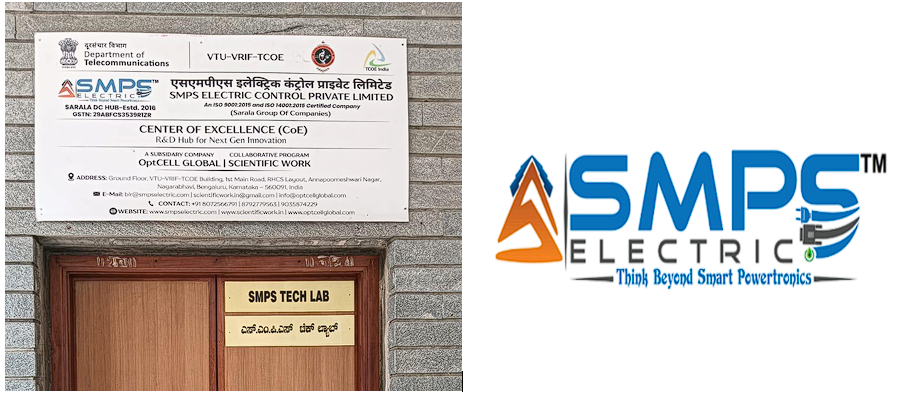
\includegraphics[width=0.8\textwidth]{office_logo.png}
\\[5mm]
\text{ Fig 1: SMPS Electric Control Pvt. Ltd. | SMPS Tech Lab}
\end{center}

\noindent
The company has a strong intellectual property portfolio with multiple innovations and patents. It has also developed indigenous semiconductor solutions, reflecting its capabilities in advanced electronics design and engineering excellence.

\subsection*{2.2 About SMPS Tech Lab}

\noindent
\textbf{SMPS Tech Lab} is the research, innovation, and technical training division functioning under SMPS Electric Control Pvt. Ltd. It serves as a platform for advanced product development, technical experimentation, and industry-oriented learning programs.

\noindent
The lab is supported by a team of engineers working in next-generation technologies such as IoT, Artificial Intelligence, Machine Learning, Industry 4.0, embedded systems, telecom technologies, renewable energy, and semiconductor design.

\begin{center}

\includegraphics[width=0.5\textwidth]{smpstechlab.png}
\\[1mm]
\text{Fig 2: SMPS Tech Lab Logo}
\end{center}
\noindent
The \textbf{Industry Fitness DeepTech Internship Program 2026} was conducted through this division to provide students with practical exposure, technical mentoring, and real-time project experience. The program was designed to prepare students for industrial expectations through structured learning and innovation-based activities.

\subsection*{2.3 Vision and Mission}

\noindent
\textbf{Vision:} To become a global leader in industrial power electronics and advanced technology solutions by promoting innovation, quality, and sustainable development.

\noindent
\textbf{Mission:} To design and deliver reliable, efficient, and high-performance engineering products that support industrial growth, uninterrupted power systems, renewable integration, and self-reliance in emerging technologies.

\noindent
The organization also aims to develop future engineers through training, internships, and research opportunities that connect academic knowledge with industrial applications.

\subsection*{2.4 Domains and Services Offered}

\noindent
The organization provides industry-specific solutions designed to meet the needs of different sectors. Its major domains include smart agriculture, industrial power electronics, corrosion protection systems, industrial field instrumentation, renewable energy systems, and smart grid or microgrid technologies.

\noindent
It also works in embedded systems, AI/ML applications, telecom technologies, IoT solutions, and industrial automation. Services include product design, prototype development, control systems, technical consultation, and skill development programs.

\noindent
Through these activities, the organization plays an important role in encouraging innovation, practical learning, and continuous technical growth while bridging the gap between academia and industry.
\newpage
\markright{OBJECTIVES OF INTERNSHIP}
\begin{flushleft}
{\fontsize{16pt}{16pt}\selectfont
\section*{CHAPTER 3}}
\end{flushleft}

\begin{center}
{\fontsize{18pt}{18pt}\selectfont \textbf{OBJECTIVES OF INTERNSHIP}}
\end{center}

\onehalfspacing
\fontsize{12pt}{14pt}\selectfont
\setlength{\parskip}{4pt}

\noindent
The internship was undertaken with the objective of providing practical exposure to industrial working methods and enhancing both technical and professional competencies. It was designed to help students apply academic knowledge in real-world situations, understand current industry practices, and develop the skills required to become industry-ready engineers. The program followed a structured dual-track learning model combining \textbf{Research \& Development (R\&D)} and \textbf{Entrepreneurship}, thereby creating a balanced platform for innovation and technical growth.

\subsection*{3.1 Technical Objectives}

\begin{itemize}
\item To gain practical exposure to an industrial and R\&D working environment and understand real-time engineering practices followed in industries.

\item To strengthen the fundamentals of electronics, digital systems, microcontrollers, and embedded systems through technical learning sessions.

\item To understand concepts related to power electronics and SMPS technology through project-based learning and system analysis.

\item To improve problem-solving ability, analytical thinking, and technical decision-making skills while working on assignments.

\item To gain exposure to engineering software tools, schematic design methods, and project execution workflow.

\item To develop innovation-oriented thinking through entrepreneurship activities and practical solution development.



\end{itemize}

\subsection*{3.2 Professional Objectives}

\begin{itemize}
\item To bridge the gap between academic learning and industry requirements.

\item To improve communication skills, teamwork, and coordination with mentors and team members.

\item To understand workplace discipline, pressure, responsibility, and professional ethics.

\item To build confidence through technical discussions, reviews, and presentations.

\item To improve adaptability, time management, leadership and readiness for future career opportunities.
\end{itemize}



\subsection*{3.3 Internship Learning Model}

\noindent
The internship followed a dual-track model that combined technical depth with innovation and business understanding. Both tracks were designed to complement each other and prepare students for real industrial challenges.

\begin{itemize}
\item \textbf{R\&D Track:} Focused on technical learning, industrial project execution, schematic understanding, system analysis, and engineering problem solving.

\item \textbf{Entrepreneurship Track:} Focused on idea generation, problem identification, market understanding, product planning, and presentation of startup-oriented solutions.

\item \textbf{Integration of Both Tracks:} Entrepreneurship develops innovation and product thinking
R\&D develops technical and analytical skills
Both tracks run in parallel and complement each other, enabling understanding of both technology development and real-world application.
\end{itemize}

\noindent
This combined learning model helped in developing technical competence, entrepreneurial mindset, leadership qualities, and industry readiness.

\begin{center}
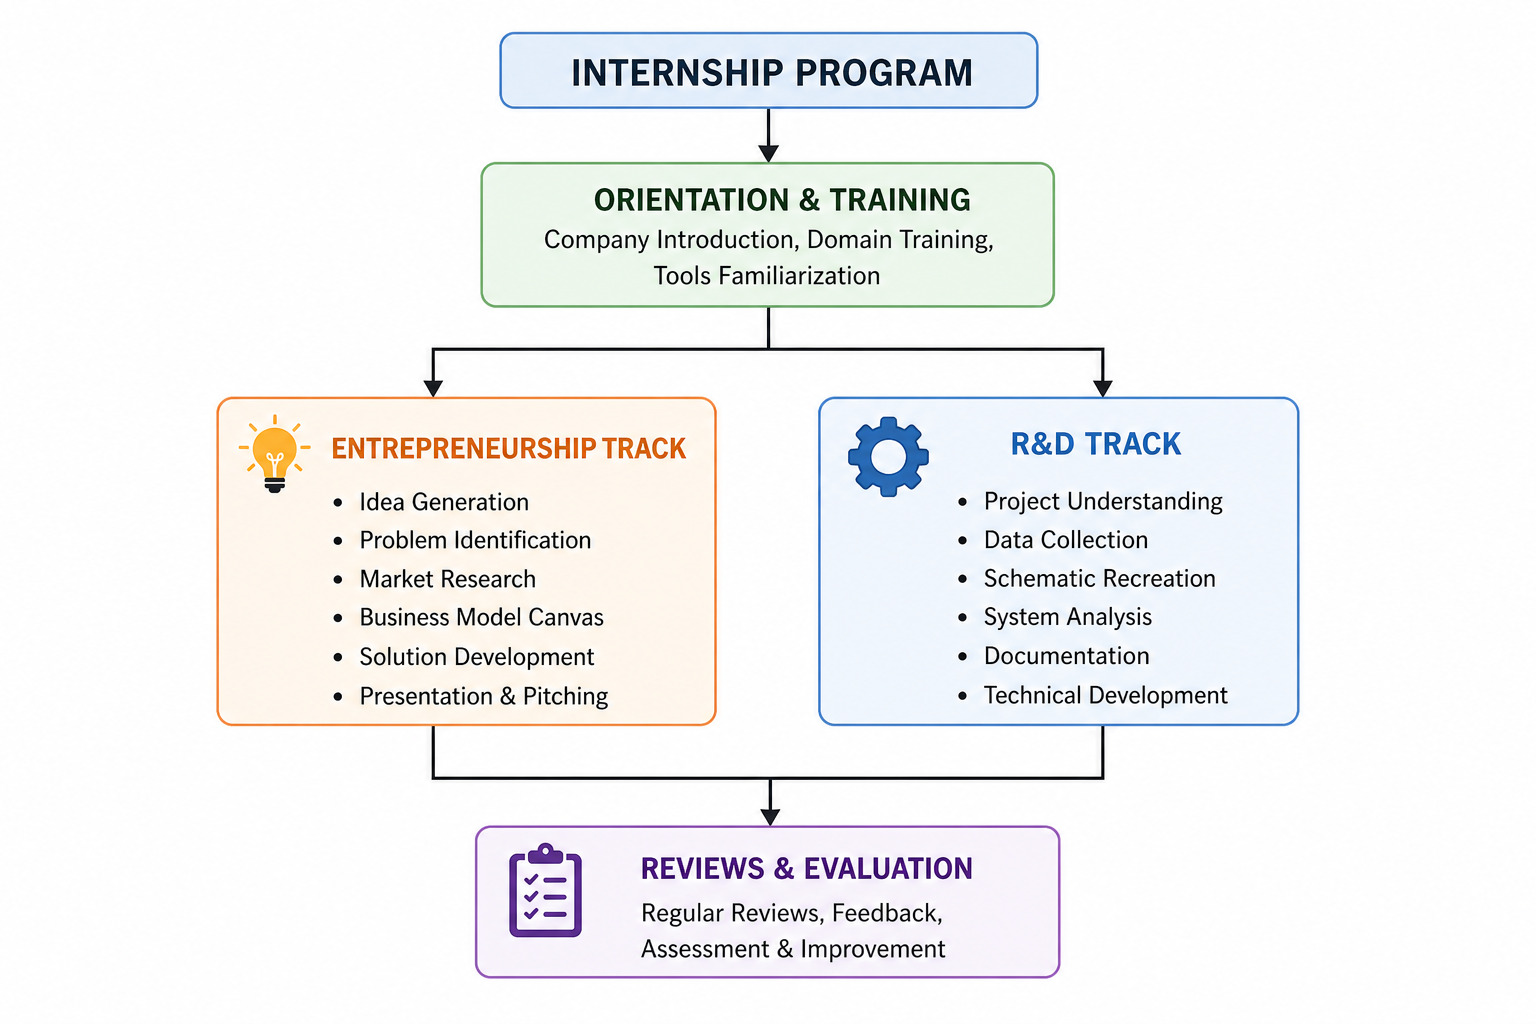
\includegraphics[width=0.99\textwidth]{flow.png}
\\[2mm]
\text{Fig 3: Internship Flow - Learning Model}
\end{center}

\newpage
\markright{WORK DONE / LEARNING EXPERIENCE}
\begin{flushleft}
{\fontsize{16pt}{16pt}\selectfont
\section*{CHAPTER 4}}
\end{flushleft}

\begin{center}
{\fontsize{18pt}{18pt}\selectfont \textbf{WORK DONE / LEARNING EXPERIENCE}}
\end{center}

\onehalfspacing
\fontsize{12pt}{14pt}\selectfont
\setlength{\parskip}{5pt}

\noindent
This chapter presents the major activities, assignments, and learning experiences carried out during the internship period. The internship provided exposure to technical training sessions, innovation-oriented project development, research and development activities, and the use of professional engineering tools. It also offered opportunities to work in a collaborative environment under the guidance of mentors and industry experts.
\subsection*{4.1 Technical and Entrepreneurship Training Sessions}
\begin{center}
% Insert training/workshop image here
\includegraphics[width=0.70\textwidth]{training2.JPG}
\\[2mm]
\text{Fig 4: Technical Training Sessions}
\end{center}
\noindent
The internship began with structured technical and professional training sessions aimed at strengthening core engineering fundamentals and preparing interns for practical industrial work. These sessions were conducted by mentors and technical experts, covering both theoretical concepts and their real-world applications.

\noindent
The major technical topics covered during the sessions included basic electronics, digital electronics, logic gates, combinational and sequential circuits, number systems, and circuit analysis. These sessions helped in refreshing academic concepts and understanding their relevance in industrial applications.

\noindent
Further sessions focused on microcontrollers and embedded systems, where concepts such as architecture, memory organization, interfacing, input-output operations, and controller-based applications were introduced. Special emphasis was given to the \textbf{8051 Microcontroller}, including its features, pin configuration, instruction concepts, and practical applications in embedded systems.

\noindent
Additional technical discussions were conducted on processor architectures such as \textbf{RISC and CISC}, ARM fundamentals, and the role of controllers in modern embedded products. These sessions helped in understanding the advancement of embedded technologies and industrial automation systems.
\begin{center}
% Insert training/workshop image here
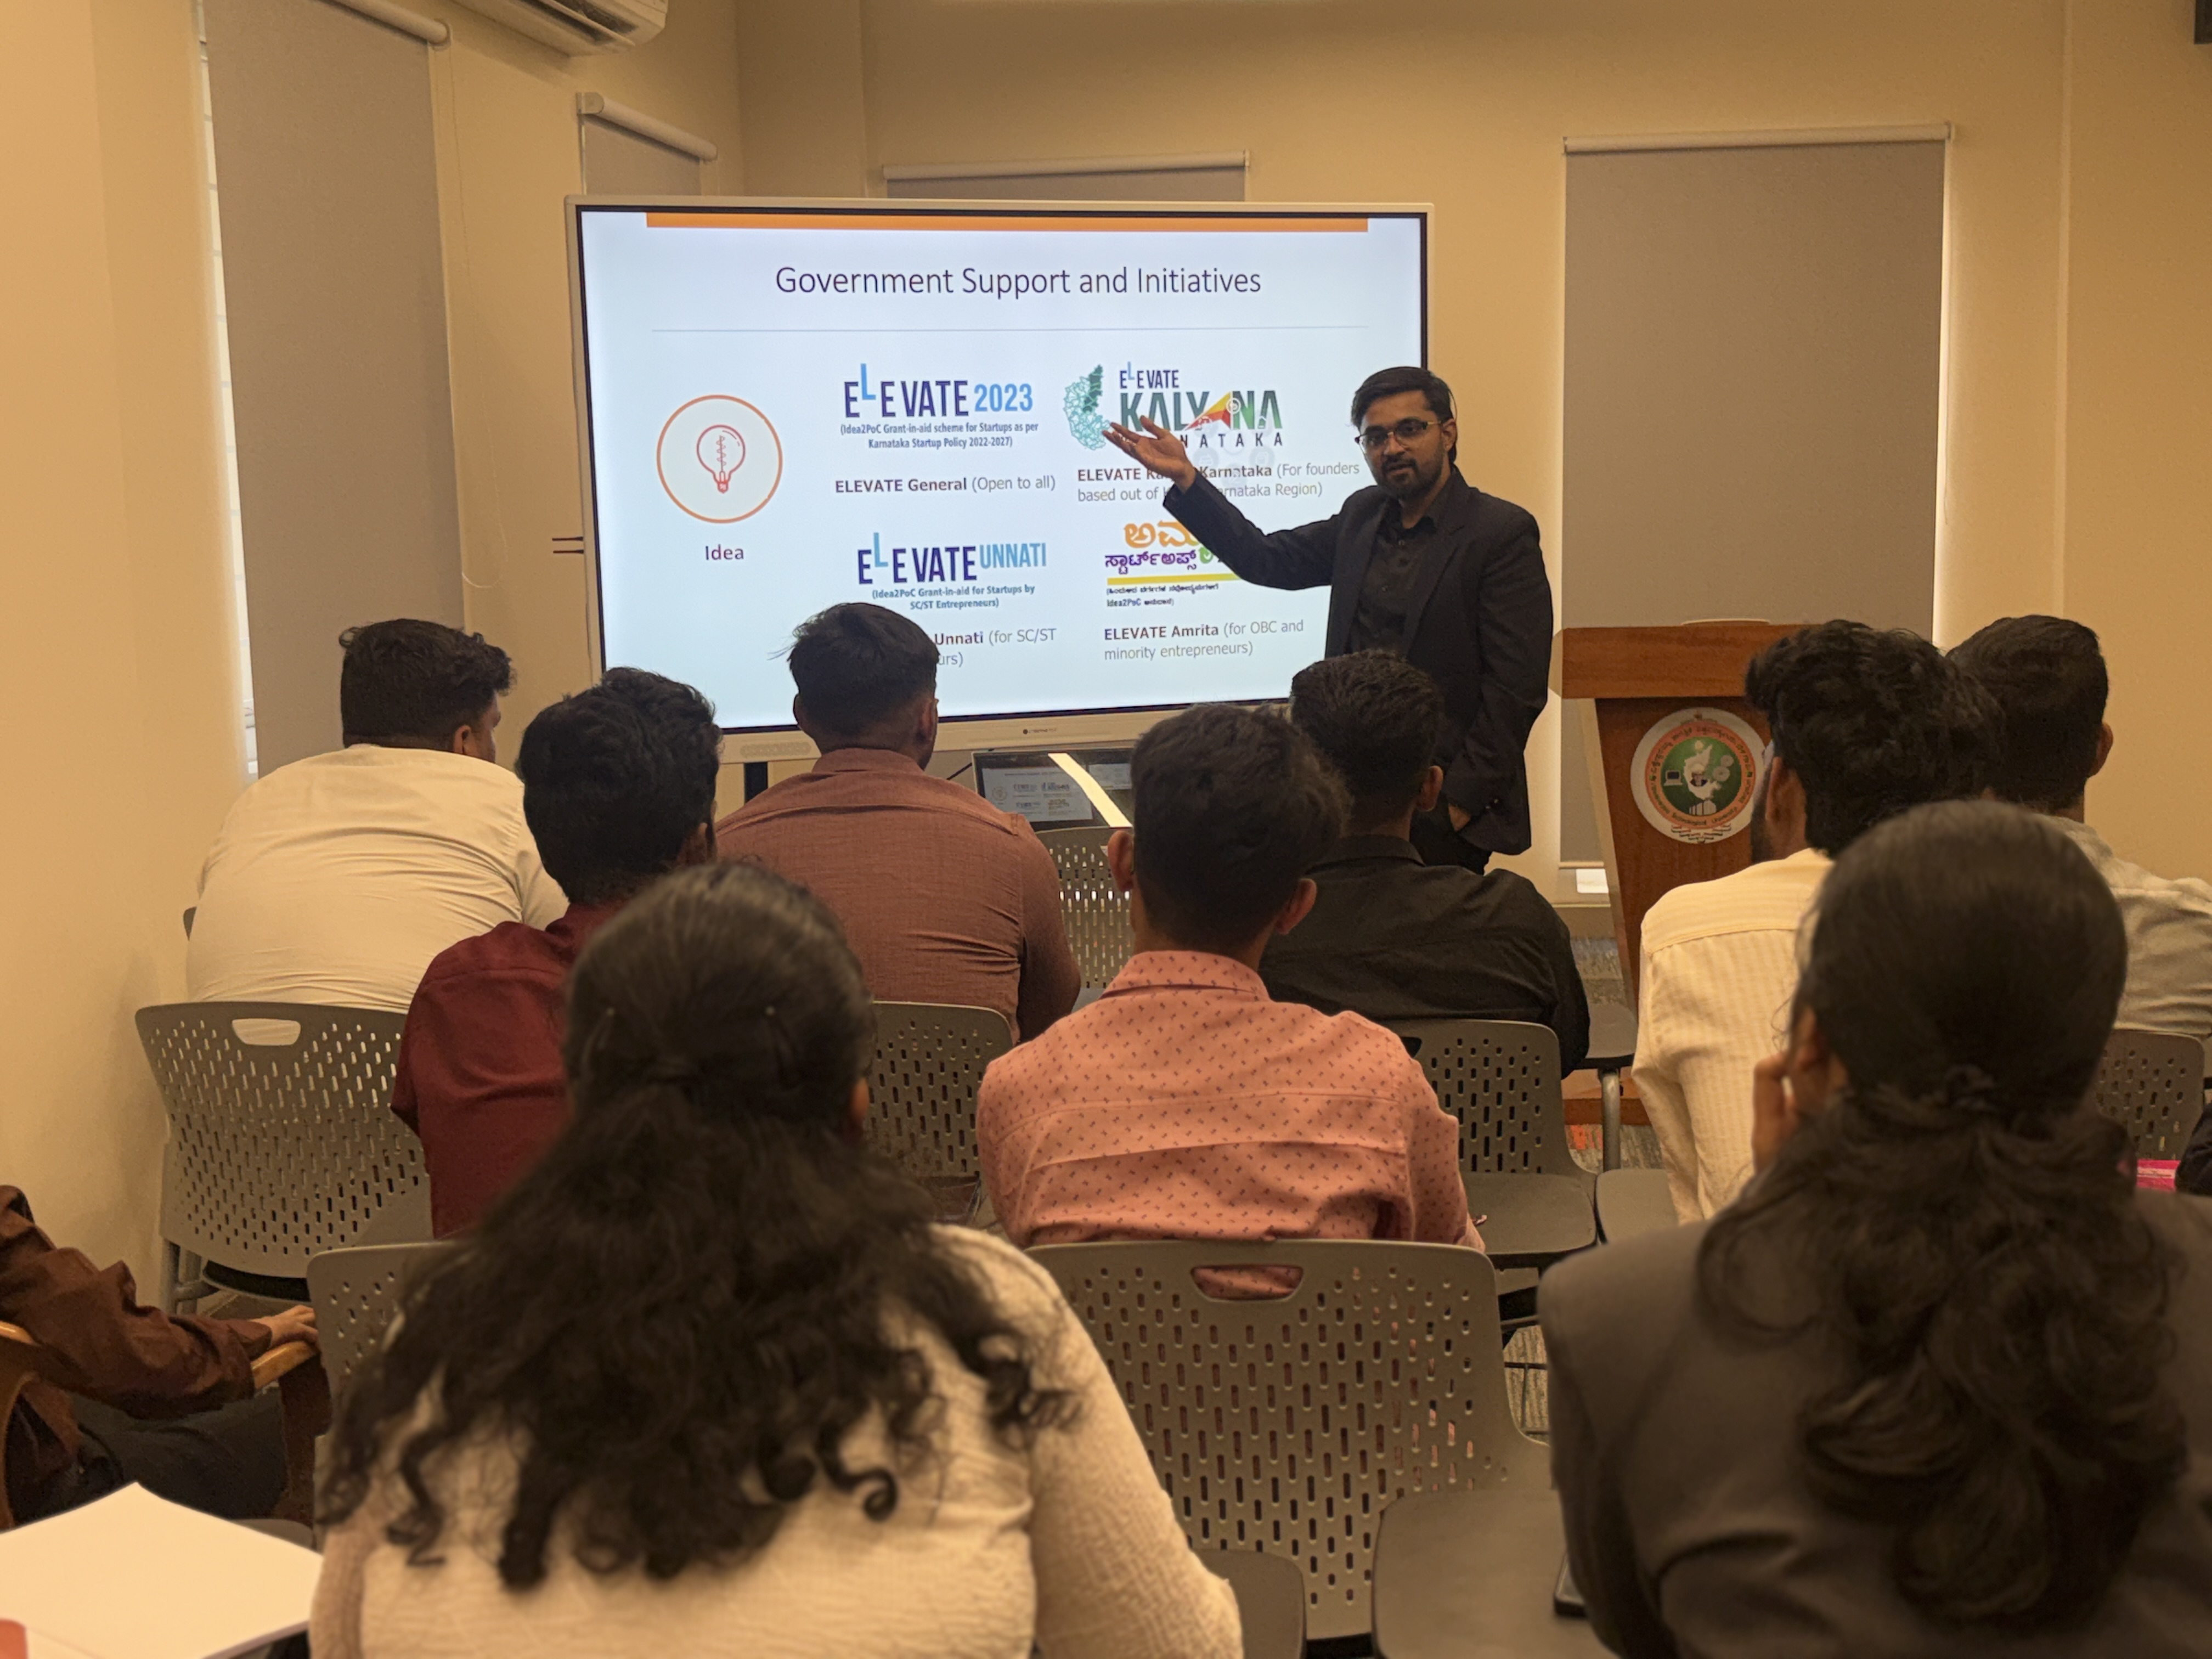
\includegraphics[width=0.90\textwidth]{training1.JPG}
\\[2mm]
\text{Fig 5: Entrepreneurship Workshop}
\end{center}
\noindent
The internship also included a two-day entrepreneurship workshop titled \textbf{Entrepreneurship Demystified}. The sessions focused on entrepreneurial mindset, identifying opportunities, solving real-world problems, and creating value through innovation. Important business concepts such as \textbf{ICP (Ideal Customer Profile)}, \textbf{SSP (Standard Sales Pitch)}, and \textbf{SOP (Standard Operating Procedure)} were introduced.

\noindent
Through these activities, interns learned that successful product development requires both technical knowledge and business understanding. The workshop also improved presentation skills, communication ability, confidence, and strategic thinking.

\noindent
As part of the final technical evaluation, emphasis was given to \textbf{8051 Microcontroller \& Embedded Systems}, covering theory, programming concepts, hardware interfacing, simulation, and practical implementation. This enhanced practical readiness and technical confidence.


\subsection*{4.2 Entrepreneurship Project -- Scan2Crack}

\noindent
As part of the entrepreneurship track of the internship,  I worked in team on a project titled \textbf{Scan2Crack -- ECE Edition}. The objective of this project was to develop a structured platform to help engineering students, especially ECE students, prepare effectively for internships and placement interviews.
\begin{center}
% Insert Scan2Crack image here
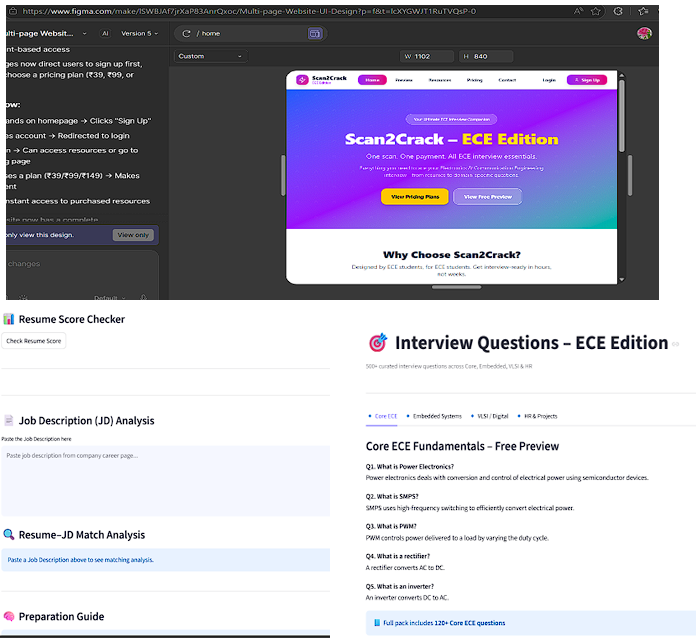
\includegraphics[width=0.52\textwidth]{scan2crack.png}
\\[2mm]
\text{Fig 6: Prototype Developed for Scan2Crack -- ECE Edition}
\end{center}
\noindent
The project was initiated after identifying a common problem faced by many students, namely the lack of proper guidance, organized preparation material, and personalized support for technical interviews. The idea was to create a platform that could simplify interview preparation in a structured and user-friendly manner.

\noindent
The proposed platform focused on providing domain-specific interview questions, resume guidance, technical preparation plans, and support for improving confidence during placements. It was designed as a student-oriented solution that could bridge the gap between academic preparation and industry expectations.
During the internship, work was carried out on idea validation, feature planning, user requirement analysis, and prototype development. Basic implementation was done using tools such as Python, Streamlit, and VS Code to demonstrate the concept through a functional MVP prototype.

\noindent
The project also provided exposure to entrepreneurship concepts such as identifying customer needs, defining value proposition, creating business models, and presenting ideas effectively. 

\noindent
This experience enhanced creativity, innovation-oriented thinking, communication skills, and confidence in presenting technical ideas as real-world solutions. It also helped in understanding that engineering knowledge can be converted into useful products and services.



\subsection*{4.3 R\&D Project -- AC-DC SMPS Power Supply}
\begin{center}
% Insert R&D project image here
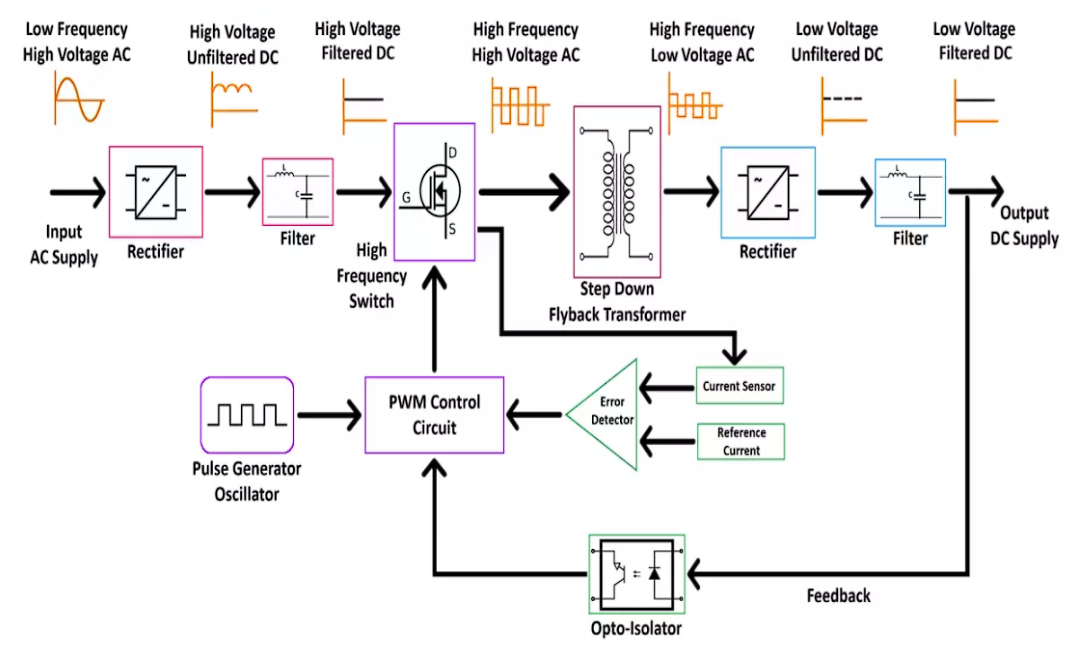
\includegraphics[width=0.65\textwidth]{rnd.png}
\\[1mm]
\text{Fig 7: AC-DC SMPS Block Diagram}
\end{center}
\noindent
As part of the Research and Development track of the internship, I worked in a team on the project titled \textbf{Forward Engineering \& Development of AC-DC SMPS Power Supply}. The project was assigned to help interns understand industrial product development methods, circuit analysis, and practical engineering workflow followed in real organizations.

\noindent
The main objective of the project was to study an existing SMPS system, understand its architecture, and analyze the important functional stages involved in power conversion. This included learning about rectification stage, DC bus formation, switching section, transformer isolation, output filtering, and feedback regulation.

\noindent
During the internship, the team carried out block-by-block study of the reference circuit and understood the purpose of various components used in the system. This activity helped in connecting theoretical concepts of power electronics with practical industrial circuit implementation.
\begin{center}
% Insert R&D project image here
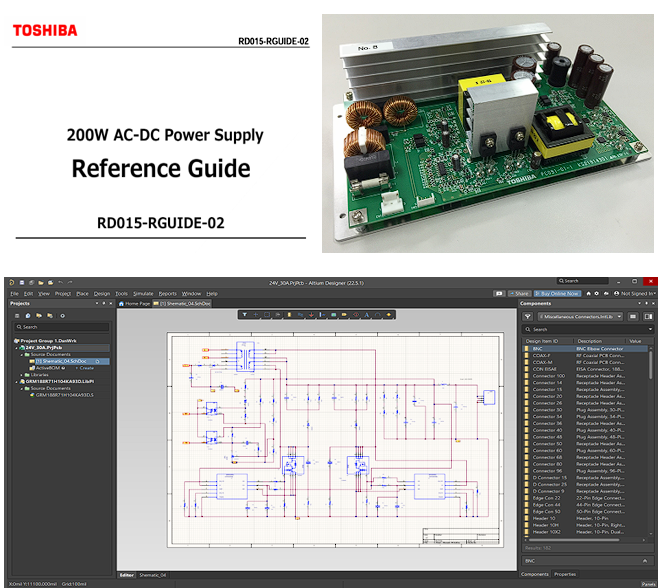
\includegraphics[width=0.48\textwidth]{rnd2.png}
\\[2mm]
\text{Fig 8: Reference and Altium Designer}
\end{center}
\noindent
Further work involved schematic recreation, component identification, footprint mapping, and understanding PCB design workflow using professional engineering tools.Exposure was also gained in reading datasheets, selecting suitable components, and studying circuit interconnections.

\noindent
The project also involved discussions on design improvement considerations such as component capability, thermal management, current handling, efficiency, and layout practices. These discussions provided insight into the practical challenges faced during real product development. Working in a team environment also enhanced collaboration, planning, and responsibility sharing skills.

\noindent
Overall, the R\&D project provided valuable exposure to industrial design methodology, research-based learning, and practical implementation concepts in the field of power electronics.

\subsection*{4.4 Tools and Technologies Used}

\noindent
The internship involved the use of various tools, software platforms, and technologies to support entrepreneurship development, technical learning, and R\&D project execution. These tools enabled efficient design, analysis, and implementation of both software-based and hardware-oriented systems.

\textbf{Development Tools (Entrepreneurship Project)}
\begin{itemize}
\item \textbf{Python} -- Used for developing application logic and backend processing.
\item \textbf{Streamlit} -- Used to build the interactive web-based interface for our project Scan2Crack platform.
\item \textbf{VS Code} -- Used as the development environment for coding and debugging.
\end{itemize}

\textbf{Design \& Engineering Tools (R\&D Project)}
\begin{itemize}
\item \textbf{Altium Designer} -- Used for schematic capture, component placement, and PCB workflow understanding.
\item \textbf{Online Component Databases} -- Used for exploring electronic components, datasheets, symbols, and footprints required for design study.
\item \textbf{Keil MicroVision} -- Used for 8051 program development, compilation, and debugging.
\item \textbf{Proteus} -- Used for simulation of embedded circuits and validation of controller-based applications.
\end{itemize}

\textbf{Learning \& Documentation Tools}
\begin{itemize}
\item \textbf{Google Drive} -- Used for maintaining daily progress reports and documentation.
\item \textbf{Microsoft Word} -- Used for preparing reports and technical documentation.
\item \textbf{Microsoft PowerPoint} -- Used for creating presentations and project reviews.
\end{itemize}

\noindent
The combination of software tools, engineering platforms, and learning resources provided balanced technical exposure and helped in becoming more industry ready.
\subsection*{4.5 Reviews, Challenges Faced and Team Participation}

\noindent
The internship included regular review meetings, progress discussions, and interactive sessions conducted by mentors and coordinators to monitor the development of assigned tasks and projects. These meetings helped in maintaining a structured workflow and ensured timely completion of activities.

\noindent
During the entrepreneurship project, review sessions were conducted to evaluate idea clarity, problem statement definition, user requirements, scalability, and presentation quality. Constructive feedback from mentors helped in refining the project concept and improving execution planning.
\begin{center}
% Insert review/team image here
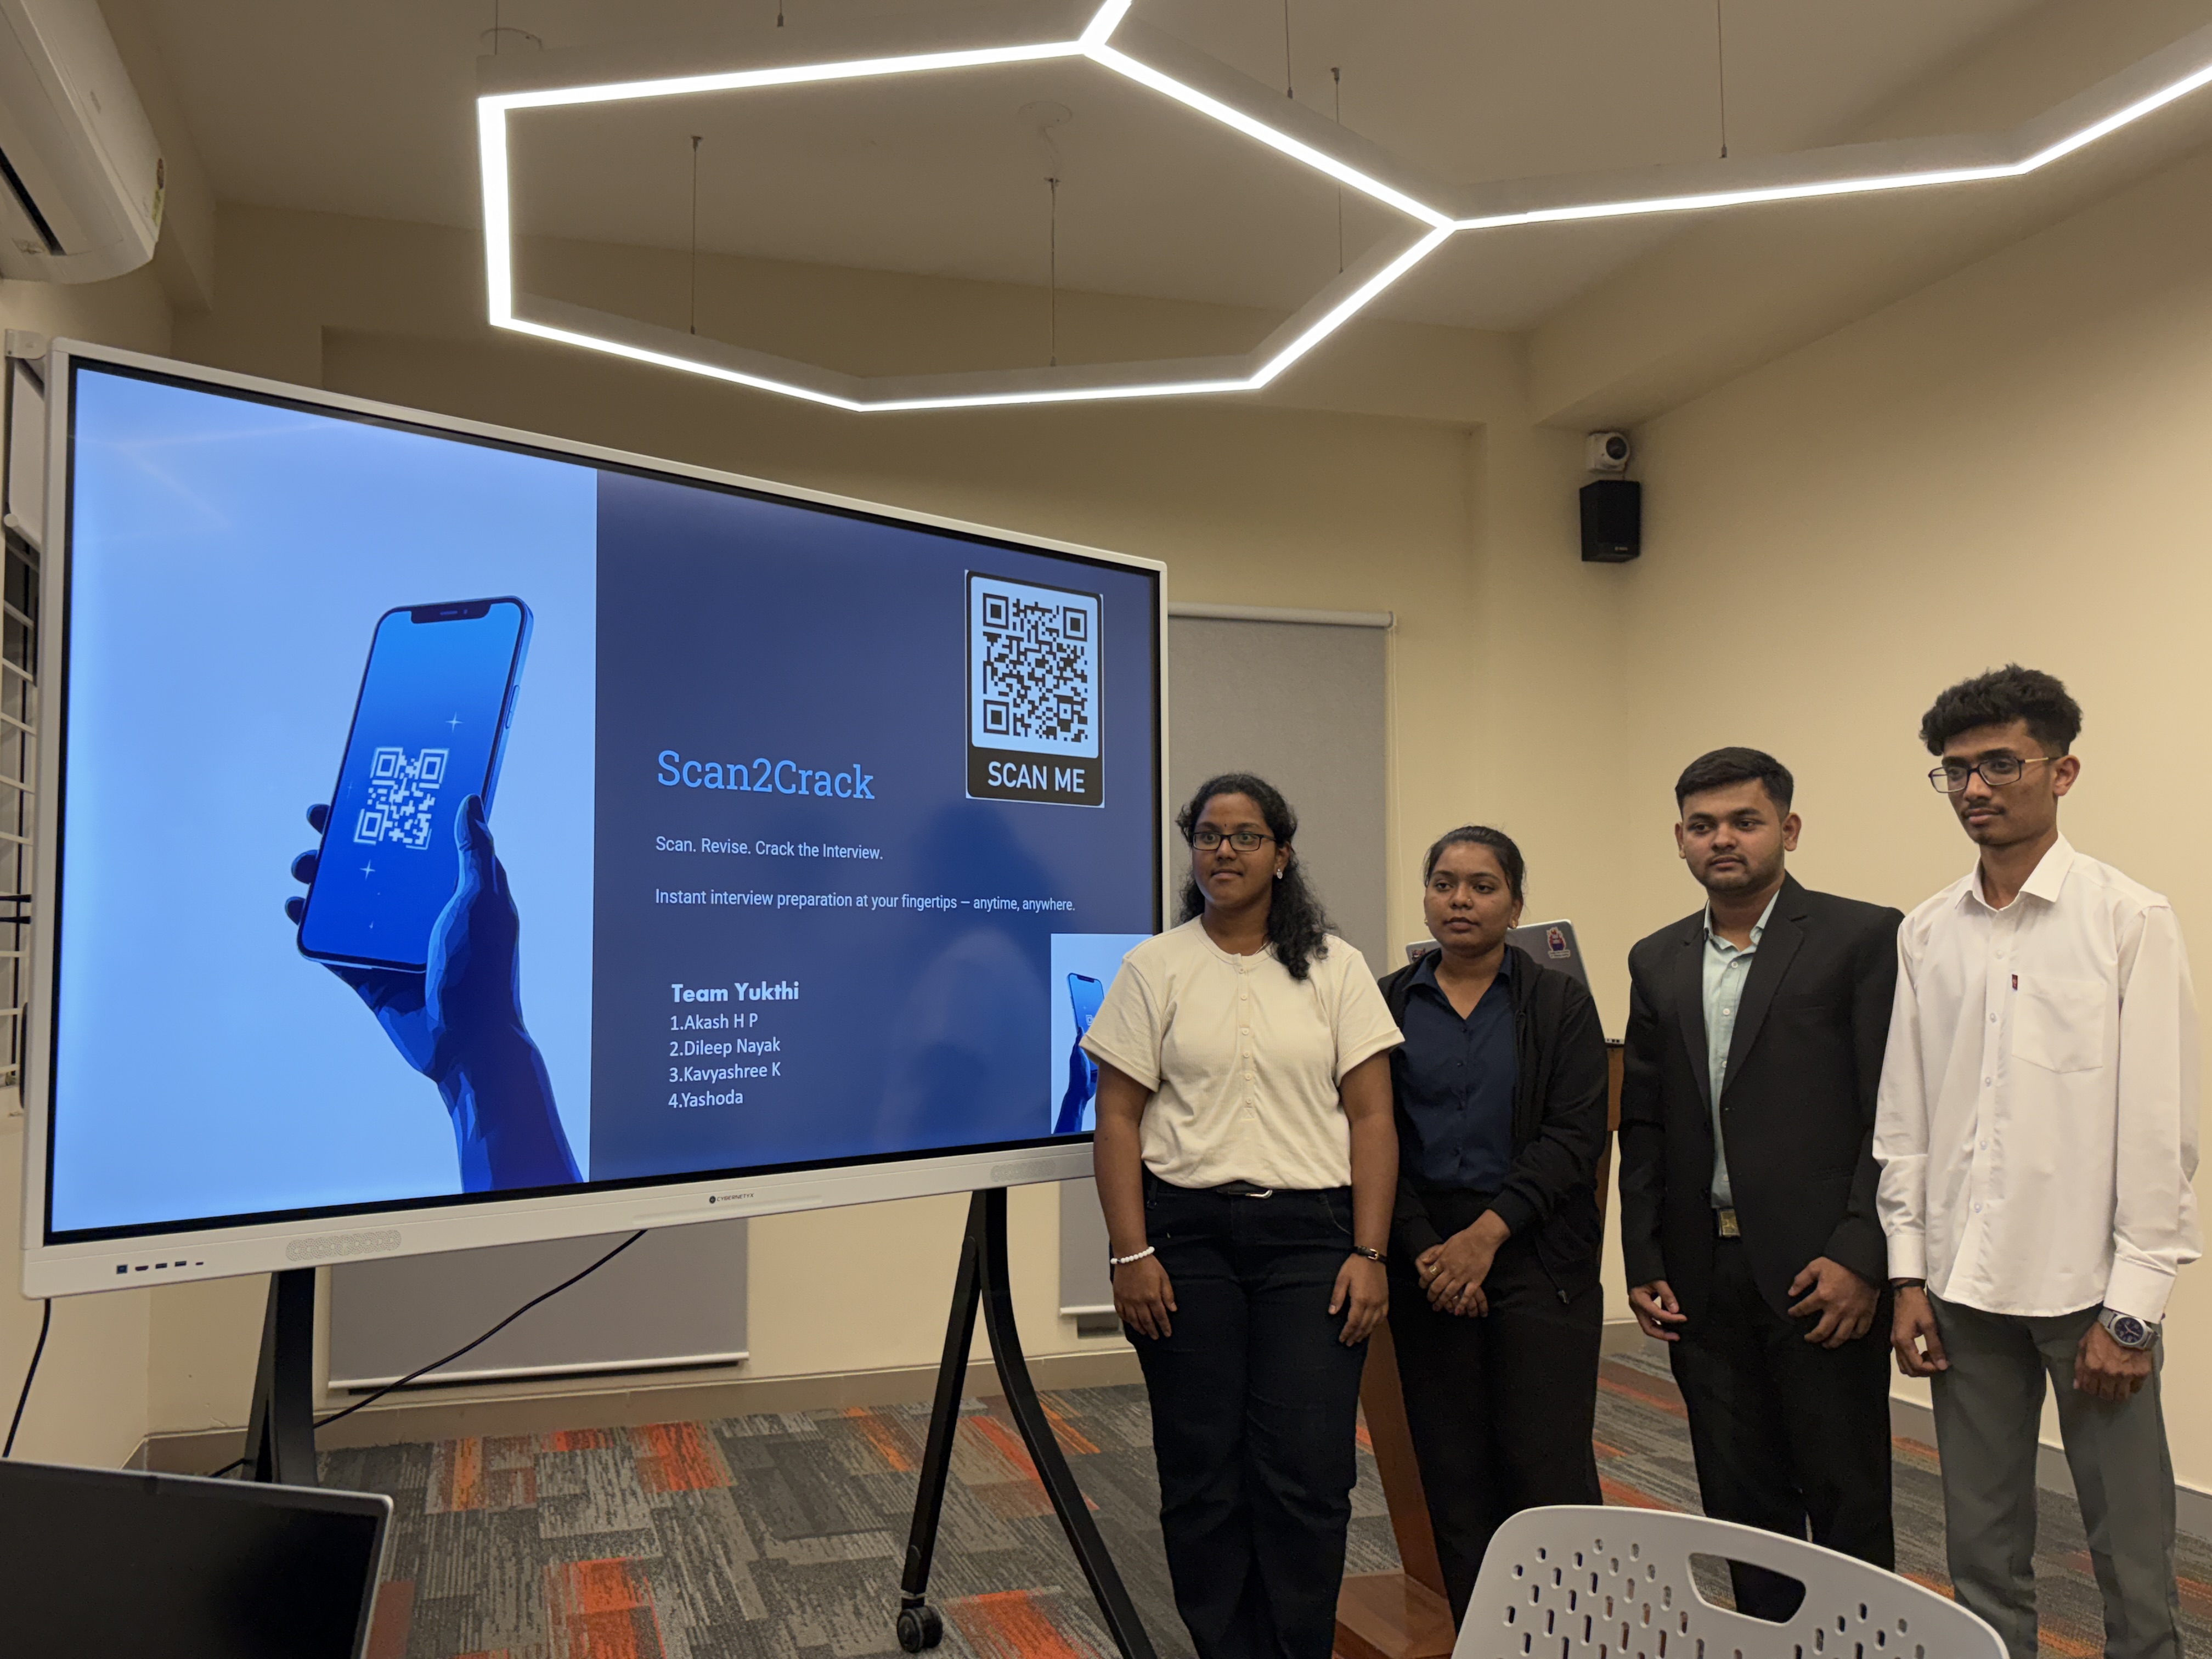
\includegraphics[width=0.85\textwidth]{review2.JPG}
\\[2mm]
\text{Fig 9: Entrepreneurship project Presentation}
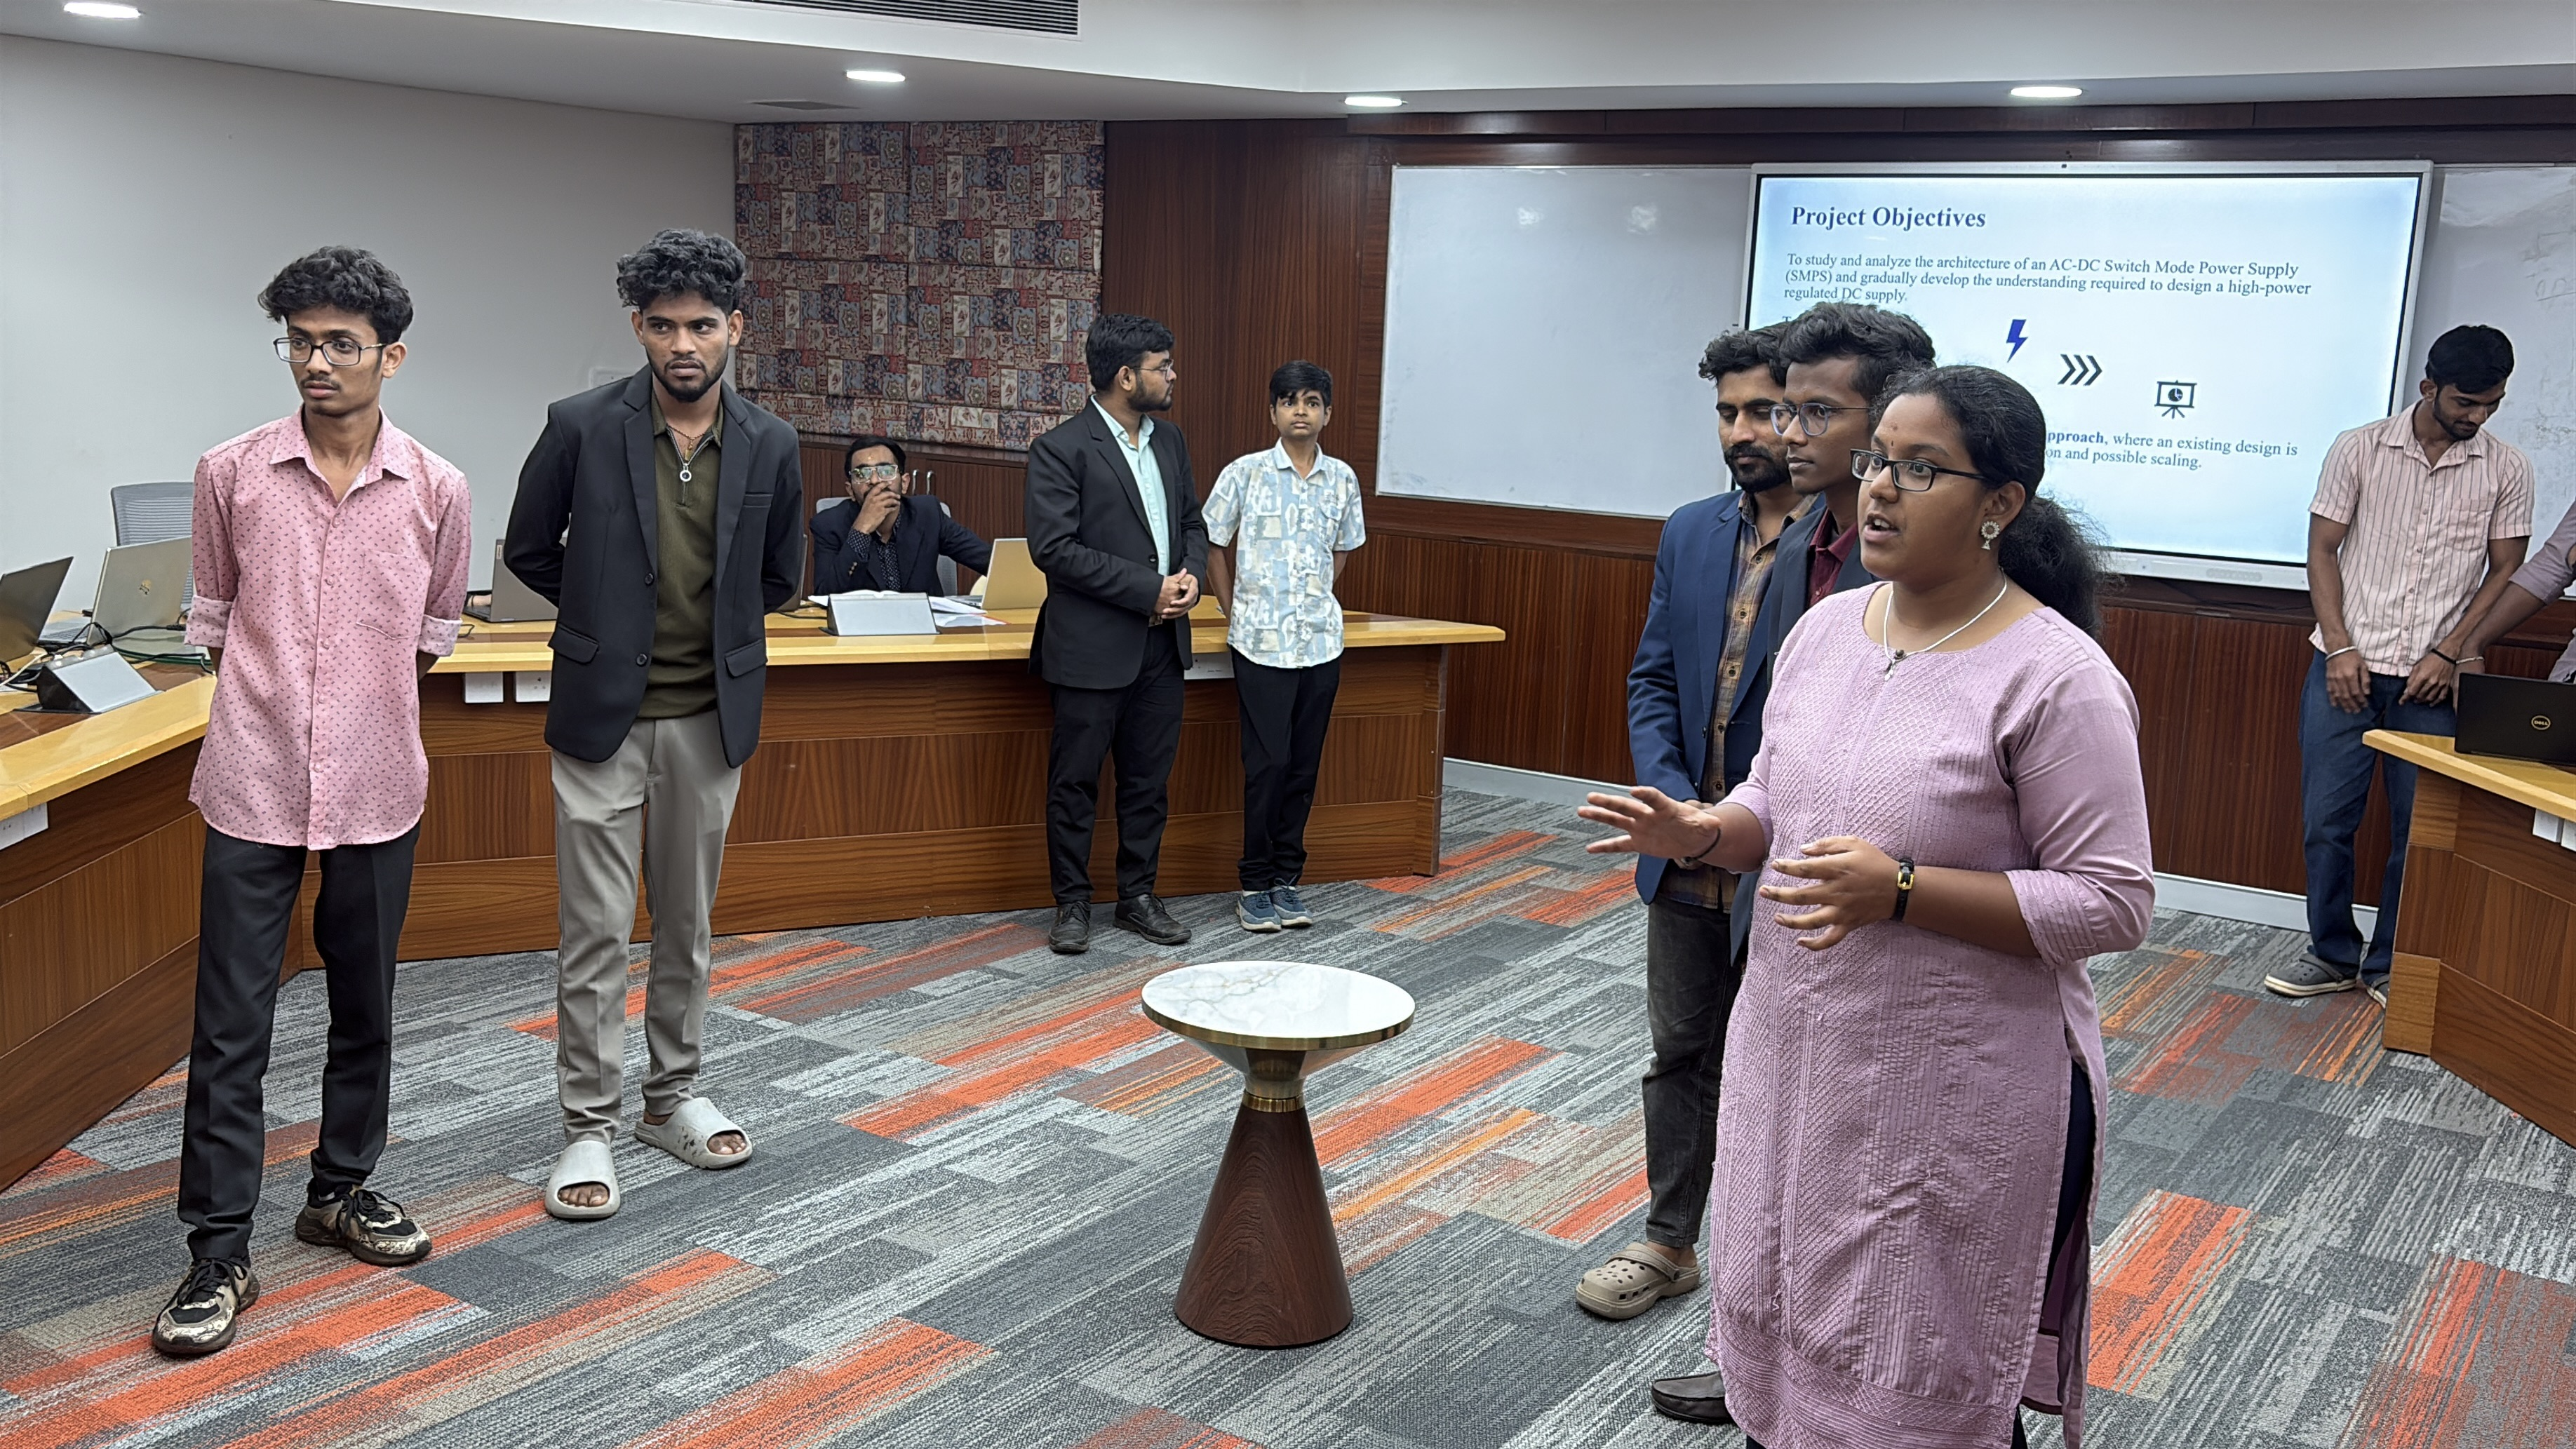
\includegraphics[width=.99\textwidth]{review1.JPG}
\\[2mm]
\text{Fig 10: R\&D Review Meeting Presentation}
\end{center}
\noindent
In the R\&D project phase, review meetings focused on technical progress, understanding of system architecture, schematic recreation status, and project planning. Guidance was provided on engineering workflow, systematic analysis, and practical problem-solving approaches.

\noindent
Some challenges faced during the internship included understanding complex industrial concepts, adapting to new software tools, managing project deadlines, coordinating team activities, and presenting ideas effectively during review sessions. These challenges were gradually overcome through continuous learning, mentor support, regular practice, and effective planning.

\noindent
The internship also involved preparation of presentations, maintenance of progress reports, and timely submission of assigned tasks. This improved documentation practices, reporting skills, and confidence in communicating technical ideas clearly.

\noindent
Working as part of a team helped in developing coordination, cooperation, leadership qualities, and responsibility sharing among members. Discussions with peers and mentors created a collaborative environment that encouraged continuous learning and improvement.

\noindent
Overall, the review sessions and team participation played an important role in enhancing communication ability, discipline, confidence, planning skills, adaptability, and professional readiness for future careers.

\newpage
\markright{LEARNING OUTCOMES}
\begin{flushleft}
{\fontsize{16pt}{16pt}\selectfont
\section*{CHAPTER 5}}
\end{flushleft}

\begin{center}
{\fontsize{18pt}{18pt}\selectfont \textbf{LEARNING OUTCOMES}}
\end{center}

\onehalfspacing
\fontsize{12pt}{14pt}\selectfont
\setlength{\parskip}{5pt}
 
\subsection*{5.1 Technical Skills Gained}
\begin{itemize}

\item \textbf{Improved understanding of electronics fundamentals, digital systems, and embedded systems:}  
Gained clarity in fundamental concepts such as logic gates, combinational and sequential circuits, and embedded system basics through structured technical sessions. This helped in strengthening core engineering knowledge and applying it in practical scenarios.

\item \textbf{Gained knowledge of 8051 Microcontroller, programming concepts, and simulation methods:}  
Developed understanding of 8051 architecture, instruction sets, and interfacing concepts. Learned to write basic programs, generate HEX files, and simulate circuits using tools like Keil and Proteus.

\item \textbf{Developed basic understanding of power electronics and SMPS system architecture:}  
Understood the working of AC-DC SMPS systems including rectification, switching, transformer isolation, and feedback mechanisms. This helped in connecting theoretical power electronics concepts with industrial applications.

\item \textbf{Learned schematic interpretation, component study, and engineering design workflow:}  
Gained the ability to read and analyze circuit schematics, identify electronic components, and understand their functions. Exposure to PCB design workflow enhanced understanding of real product development processes.

\item \textbf{Gained exposure to software tools such as Python, Streamlit, Keil MicroVision, and design platforms:}  
Used Python and Streamlit for developing a basic web-based prototype, and Keil and Proteus for embedded system development and simulation. This improved familiarity with industry-relevant tools.

\item \textbf{Improved analytical thinking and technical problem-solving ability:}  
Enhanced the ability to analyze engineering problems, break them into smaller parts, and develop logical solutions through continuous practice and project work.

\end{itemize}


\subsection*{5.2 Professional Skills Developed}
\begin{itemize}
\item \textbf{Improved communication skills through presentations, reviews, and discussions:}  
Actively participated in technical discussions and project presentations, which helped in improving clarity of expression and confidence in communicating ideas effectively.

\item \textbf{Developed teamwork and coordination while working on group projects:}  
Worked collaboratively with team members, shared responsibilities, and contributed to project execution. This improved coordination, cooperation, and interpersonal skills.

\item \textbf{Understood workplace discipline, responsibility, and professional ethics:}  
Learned the importance of punctuality, accountability, and maintaining professional behaviour in an industrial environment.

\item \textbf{Improved time management and ability to work under deadlines:}  
Managed multiple tasks and project deadlines efficiently, which helped in improving planning, prioritization, and execution skills.

\item \textbf{Built confidence in presenting ideas and interacting in professional environments:}  
Regular reviews and presentations enhanced confidence in explaining technical concepts and interacting with mentors and professionals.

\end{itemize}


\subsection*{5.3 Industry Exposure}
\begin{itemize}

\item \textbf{Understood how industries plan, execute, and review technical projects:}  
Gained insight into structured project workflows, including planning, development, testing, and evaluation processes followed in industries.

\item \textbf{Gained awareness of industrial tools, workflows, and documentation practices:}  
Learned how professional tools and documentation methods are used to maintain accuracy, consistency, and traceability in engineering projects.

\item \textbf{Learned the importance of innovation, entrepreneurship, and market-oriented thinking:}  
Through the entrepreneurship track, understood how technical ideas can be converted into practical products by considering user needs and market demands.

\item \textbf{Experienced mentor guidance and collaborative work culture:}  
Worked under the guidance of experienced mentors, which helped in improving learning efficiency and understanding industry expectations.

\item \textbf{Developed industry readiness by understanding workplace expectations, technical standards, and professional practices:}  
Gained awareness of quality standards, technical precision, and professional conduct required in real-world engineering environments.

\item \textbf{Developed readiness for future internships, placements, and engineering careers:}  
The overall exposure improved confidence, technical competence, and preparedness for future career opportunities in engineering domains.

\end{itemize}


\newpage
\markright{CONCLUSION}
\begin{flushleft}
{\fontsize{16pt}{16pt}\selectfont
\section*{CHAPTER 6}}
\end{flushleft}

\begin{center}
{\fontsize{18pt}{18pt}\selectfont \textbf{CONCLUSION}}
\end{center}

\onehalfspacing
\fontsize{12pt}{14pt}\selectfont
\setlength{\parskip}{6pt}

\noindent
The Industry Fitness DeepTech Internship Program 2026 at SMPS Tech Lab under SMPS Electric Control Pvt. Ltd. was a highly valuable and enriching learning experience. The internship successfully bridged the gap between academic knowledge and practical industrial applications by providing exposure to real-time engineering practices, technical projects, and professional work culture.

\noindent
During the internship, I gained knowledge in electronics fundamentals, embedded systems, microcontrollers, power electronics, and engineering workflow through structured technical sessions and project-based learning. Special focus on 8051 Microcontroller \& Embedded Systems further enhanced my understanding of controller programming, simulation, and practical implementation concepts.

\noindent
The entrepreneurship activities and the \textbf{Scan2Crack -- ECE Edition} project helped in developing creativity, innovation-oriented thinking, communication skills, and problem-solving ability. The R\&D project on \textbf{AC-DC SMPS Power Supply} provided useful exposure to industrial design methodology, system analysis, and technical teamwork.

\noindent
The internship also improved my confidence, teamwork, time management, presentation skills, and awareness of industry expectations. It enabled me to understand the importance of continuous learning, adaptability, and professionalism in engineering careers.
\noindent
The knowledge and experience gained during this internship can be further developed through advanced project implementation, deeper research in embedded systems and power electronics, and continued learning of industrial tools. The internship has motivated me to explore future opportunities in core engineering domains, innovation-based projects, and professional career growth.

\noindent
Overall, the internship was a significant step in my academic and professional growth. It prepared me to face future career opportunities with better technical competence, industry readiness, and a positive learning attitude.\\

\noindent
\textbf{Future Scope:} The knowledge and experience gained during this internship can be further enhanced through advanced project implementation, deeper research in embedded systems, power electronics, and industrial automation. The exposure received in entrepreneurship and R\&D activities has motivated me to explore future opportunities in core engineering domains, innovation-driven projects, and continuous professional development.

\newpage
\markright{REFERENCES}
\begin{flushleft}
{\fontsize{16pt}{16pt}\selectfont
\section*{REFERENCES}}
\end{flushleft}

\onehalfspacing
\fontsize{12pt}{14pt}\selectfont
\setlength{\parskip}{6pt}

\begin{enumerate}

\item Massachusetts Institute of Technology (MIT), ``Power Electronics (6.622, Spring 2023),'' MIT OpenCourseWare.

\item SMPS Tech Lab, Internship learning materials, technical notes, project guidance resources, and internal training sessions provided during the internship period.

\item YouTube Learning Resources referred for understanding embedded systems, SMPS working principles, entrepreneurship concepts, and technical software tutorials.

\item Keil Software, ``Keil MicroVision IDE,'' used for learning 8051 microcontroller programming and embedded system development.

\item Altium Limited, ``Altium Designer,'' used for schematic capture and PCB design workflow understanding.

\item Streamlit Inc., ``Streamlit Documentation,'' referred for web-based prototype development during the Scan2Crack project.

\item Python Software Foundation, ``Python Documentation,'' referred for programming concepts and application development.

\item Microsoft Corporation, ``Microsoft Word and PowerPoint,'' used for report preparation, presentations, and documentation.

\item Mentor guidance, review meetings, discussions, and practical demonstrations conducted by experts during the Industry Fitness DeepTech Internship Program 2026.

\end{enumerate}
\end{document}